\newtheorem{fig}{\vspace{-10pt} Figure}
\newtheorem{tab}{\hspace{-5pt} Table}

\def \dt{\Delta t}
\def \dz{\Delta z}
\def \eps{\varepsilon}
\def \degrees{^\circ}

\def \bc{\begin{center}}
\def \ec{\end{center}}
\def \be{\begin{equation}}
\def \ee{\end{equation}}
\def \ba{\begin{array}}
\def \ea{\end{array}}
\def \bt{\vspace{2mm} \begin{tabular}}
\def \et{\end{tabular}}
\def \bd{\begin{displaymath}}
\def \ed{\end{displaymath}}
\def \bi{\begin{itemize}}
\def \ei{\end{itemize}}
\def \ben{\begin{enumerate}}
\def \een{\end{enumerate}}
\def \bc{\begin{center}}
\def \ec{\end{center}}
\def \di{\displaystyle}

\def \bgf{\begin{figure} \bc}
\def \bgfh{\begin{figure}[h] \bc}
\def \bgft{\begin{figure}[t] \bc}
\def \bgfb{\begin{figure}[b] \bc}
\def \bgfht{\begin{figure}[ht] \bc}
\def \bgfhb{\begin{figure}[hb] \bc}
\def \ef{\ec \end{figure}}

\def \btb{\begin{table} \bc}
\def \btbh{\begin{table}[h] \bc}
\def \btbht{\begin{table}[ht] \bc}
\def \etb{\ec \end{table}}

\chapter{Model Description}
The sea ice model is based on the zero layer model of
 \cite{semtner1976}. This model
 computes the thickness of the sea ice from the thermodynamic
 balances at the top and the bottom of the sea ice.
 The zero layer assumes the temperature gradient in the ice to
 be linear and eliminates the capacity of the ice to store heat.
 Nevertheless, it has been used successfully in areas where ice
 is mostly seasonal and thus relatively thin ($\rm <\, 1\, m$)
 \cite{beckmann2001}.
 Thus, the model is expected to perform better in the Southern
 Ocean than in the Arctic, where multiyear, thick ice dominates
 (cf. section 'Validation'). Sea ice is formed if the ocean
 temperature drops below the freezing point
 (271.25 K, cf. Eq. (\ref{tfeq})) and is melted whenever the
 ocean temperature increases above this point. The prognostic
 variables are the sea ice temperature $T_i\, \rm (K)$, the ice
 thickness $h_i \, \rm (m)$ and the ice concentration $A$, which
 in the present model is boolean: A given grid point is either
 ice free ($A=0$) or ice covered ($A=1$). The freezing
 temperature $T_f\, \rm(K)$ depends on salinity as
 \cite{unesco1978}
\be
T_f\, =\, 273.15\, -0.0575S_w\, +1.7105\times 10^{-3}S_w^{3/2}\, -2.155\times 10^{-4}S_w^2,
\label{tfeq}
\ee
where $S_w\,\rm(psu)$ denotes the salinity of sea water.
 On the range $0 \,<\, S_w \,<\, 40$, the salinity
 - freezing point dependency reduces to a linear relationship
 where $T_f$ decreases with increasing salinity.

Freezing and melting of sea ice releases just the right amount of latent heat 
of fusion to close the energy balance with respect to the total heat flux
$Q \, \rm (W\, m^{-2})$ in the mixed layer \cite{parkinson1979}:
\be
Q\, +\rho_i\, L_i\, \frac{dh_i}{dt} =\, 0,
\label{hieq}
\ee
where $\rho_i\, \rm (kg\, m^{-3})$ is the density of sea ice
 and $L_i\, \rm (W\, m^{-1}\, K^{-1})$ denotes the latent heat
 of fusion of sea ice. Standard parameter values are given in
 Table \ref{iceparatab}. \cite{parkinson1979} Thus, the prognostic
 equation for the sea ice thickness is given as
\be
{\di \frac{dh_i}{dt} = \frac{-Q}{\rho_i \, L_i}.}
\label{hi_eq}
\ee
It is assumed that melting of sea ice takes place from above only, while 
freezing takes place at the lower side of the ice floe.

\bgfht
\def\epsfsize#1#2{0.5#1}
\vspace{-3cm}
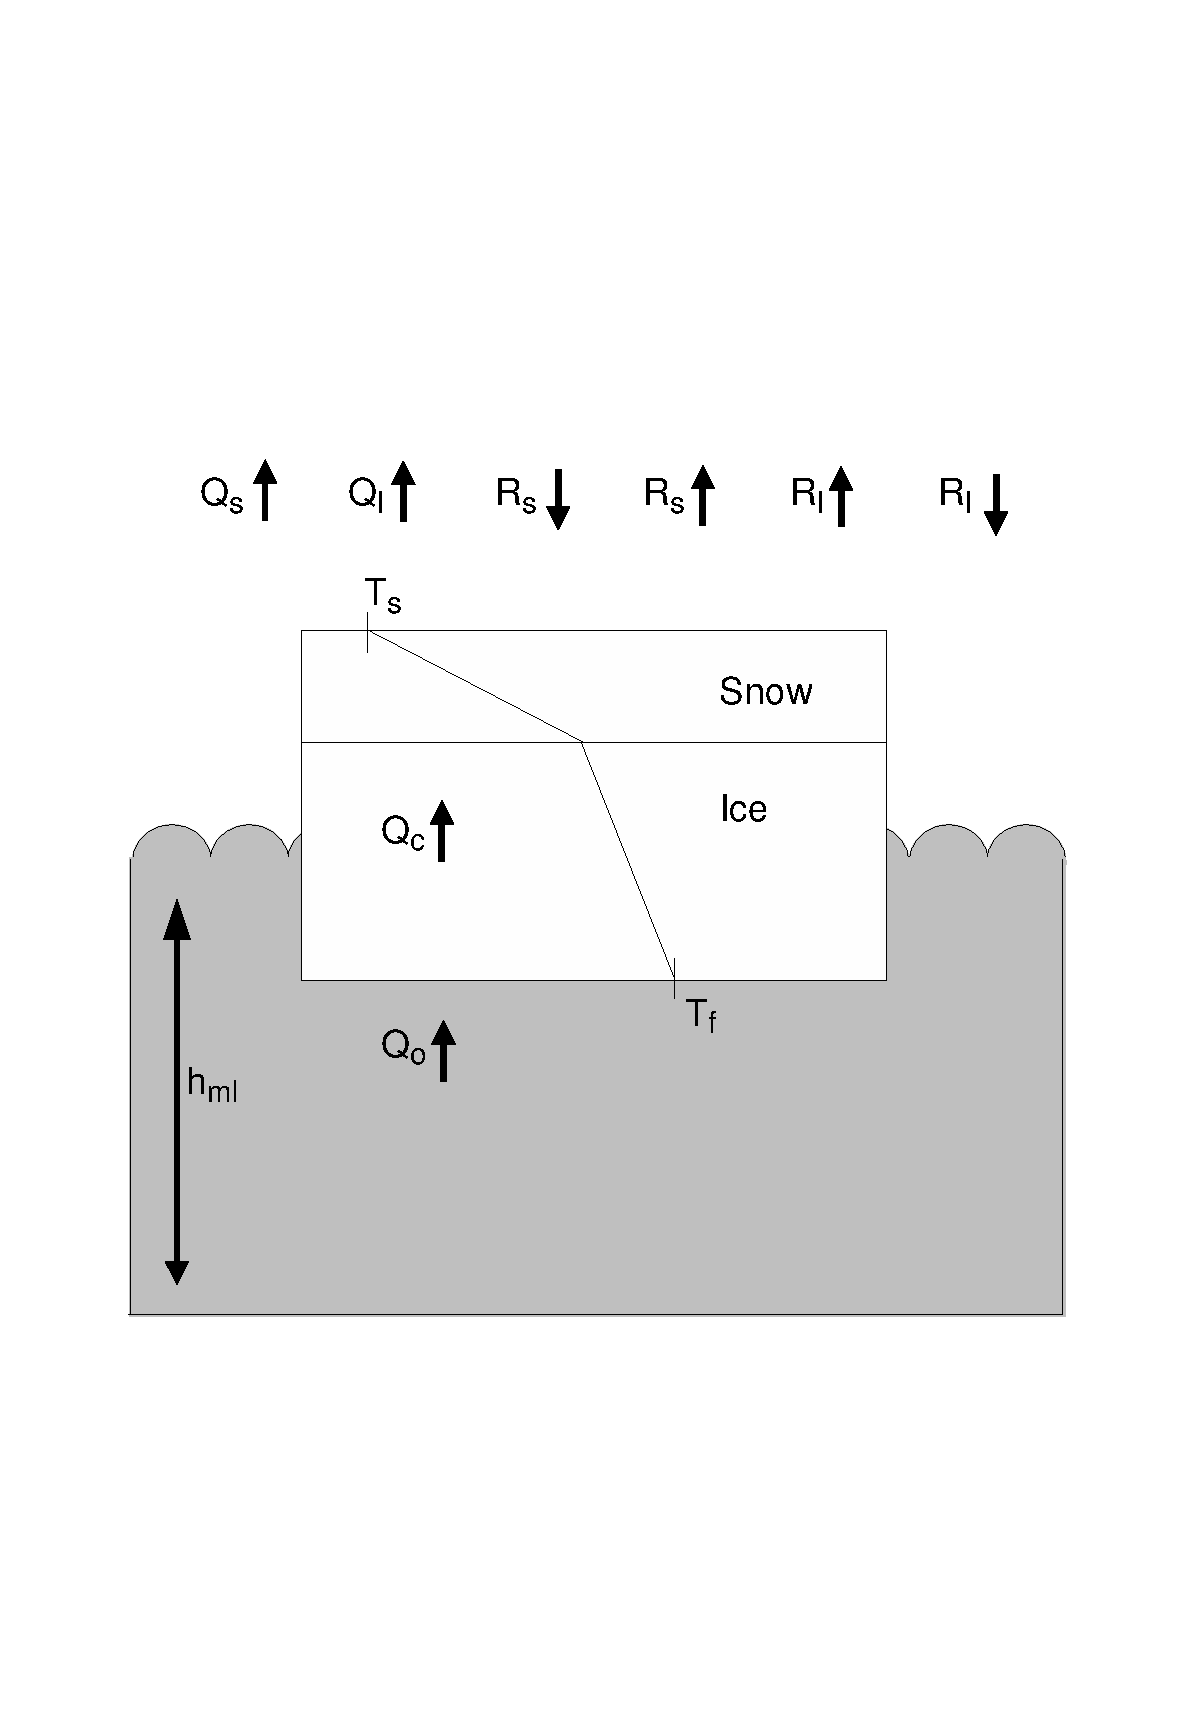
\includegraphics[width=13cm]{heiko/modules_icemod_schema}
%\centerline{\vbox{\epsfbox{heiko/modules_icemod_schema.ps}}}
\vspace{-3cm}
\caption{Schematic illustration of the temperature profile in the sea ice and
the relevant heat fluxes. The atmospheric heat flux is the sum of sensible and
latent heat flux ($Q_s,\,Q_l$), the incoming and reflected short wave 
radiation ($R_{s,\downarrow}\, R_{s,\uparrow}$) and the long wave radiation 
($R_l$). Ice growth and melting processes are additionally influenced by the 
conductive heat flux $Q_c$ through the ice floe and the oceanic heat flux 
$Q_o$ resulting from the temperature difference between water and ice.
The mixed layer depth $h_{ml}$ determines how much energy is available for ice 
formed from open water. The bottom temperature of the ice floe is set to the 
freezing temperature $T_f$. The sea ice surface temperature $T_s$ is 
calculated according to the energy balance at the surface.}
\label{schemafig}
\ef


\section*{Basic equations}
In the presence of sea ice, the heat fluxes are defined as follows.
The total heat flux $Q\, \rm (W\, m^{-2})$ is given as
\be
Q \,=\, Q_a\, +Q_c\, +Q_o\, +\tilde{Q},
\ee
where $Q_a$ is the atmospheric heat flux,
$Q_c$ is the conductive heat flux through the ice, $Q_o$ denotes the oceanic 
heat
flux and $\tilde{Q}$ is the flux correction. The atmospheric heat flux
\be
Q_a = \left\{ \ba{lcr}
\, F_T\, +L\, +R_{s,\downarrow}\, +R_{s,\uparrow}\,
	+R_{l,\downarrow}\, +R_{l,\uparrow}\, & {\rm if} & T_s > T_f, \\
0 & {\rm if} &  T_s \le T_f.
\ea \right. \label{qa_eq}
\ee
is the sum of sensible ($F_T$) and latent heat flux ($L$), the incoming and
reflected short wave radiation ($R_{s,\downarrow}\, R_{s,\uparrow}$)
and the long wave radiation ($R_l$). It is set to zero in the case of freezing,
where the conductive heat flux applies (see below).
The conductive heat flux through the ice
\be
Q_c = \left\{ \ba{lcr}
0 & {\rm if} & T_s > T_f, \\
{\di \frac{\bar{\kappa}}{h_i\, +h_s}\, (T_s -T_f)} & {\rm if} &  T_s \le T_f.
\ea \right. \label{qc_eq}
\ee
is set to zero in the case of melting ice, as the ice melts at the top. If the 
ice is freezing, the atmospheric heat flux determines the surface temperature 
$T_s$ and has to pass through the ice. Whatever energy is left at the
 bottom of the ice sheet is then available for freezing.
 $\bar{\kappa}\, \rm (W\, m^{-1}\, K^{-1})$ is the mean conductivity
 of the sea ice floe and snow cover, computed as
\be 
{\di \bar{\kappa}\, =\, \frac{\kappa_i h_i\, +\kappa_s h_s}{h_i\, +h_s}}.
\ee
The oceanic heat flux is considered only in the presence of sea ice:
\be
Q_o\, =\, c_o\, (T_d\, -T_f).
\label{qoce} \ee
It is determined by the gradient between the temperature of sea water in the 
deep
ocean ($T_d,\, \rm (K)$) and the surface temperature, which is the
freezing temperature ($T_f,\, \rm (K)$). In the absence of sea ice, the oceanic
heat flux is implicitly considered as it determines the sea water temperature
in the mixed layer ($T_s,\, \rm (K)$). 
The flux correction is calculated as
\be
{\di \tilde{Q}\, =\, \frac{\rho_i\, L_i}{\eps_c}\, (h_i\, -h_{i,c}),}
\ee
where $h_{i,c}\, \rm (m)$ is the climatological ice thickness and $\eps_c$ is a
relaxation constant. For example, $\eps\, =\, 2000$ corrects the ice thickness
to climatological values in 2000 time steps.

In the case of melting ice, the ice thickness may become negative if the 
energy available for melting is greater than needed to
 melt the present ice. Then, the surplus energy is heating the
 sea water, setting the surface temperature to
\be
{\di T_s\, =\, T_f\, -\frac{\rho_i\, L_i\, h_i}{\rho_w\, c_{p_s}\, h_{mix}} },
\ee
with $h_i < 0$.

\section*{Ice formation from open water}
If the surface temperature of open ocean water is below the freezing point,
sea ice is formed. The heat flux available for freezing is given as
\be
Q_f\, =\, {\di \frac{\rho_w\, c_{p_w}\, h_{ml}}{dt} \, (T_s\, -T_f)\, 
+Q_{next},}
\ee
where $\rho_w\, \rm(kg\, m^{-3})$ is the density of sea water,
$c_{p_w}\, \rm(W\, s\, kg^{-1}\, K^{-1})$ is the specific heat of sea water and
$h_{ml}\, \rm(m)$ denotes the mixed layer depth. The thickness of the new 
formed
ice sheet is calculated by setting $Q\, =\, Q_f\, +\tilde{Q}$
in (\ref{hieq}). We have prescribed a
minimum ice thickness $h_{i,min}\, =\, 0.1\, \rm m$, since the presence of sea
ice drastically changes the albedo. Open ocean has an albedo of 0.1, whereas 
sea
ice yields an albedo of 0.7. As the model differentiates only between no ice 
and
full ice in one gridpoint, the albedo would change unrealistically early in 
the case
of ice formation without the prescribed minimum thickness. If less than 10 cm 
ice
is formed in one time step, the flux to form this amount of ice is taken to the
next time step.Thus,
\be
Q_{next} = \left\{ \ba{rcl}
0 & {\rm if} & h_i \ge 0.1, \\
Q_f & {\rm if} &  h_i < 0.1.
\ea \right.
\ee
If, for example, 4 cm ice is formed per time step and conditions
do not change, it takes three time steps until the grid point is classified as
ice covered.


\section*{Sea ice temperature}
The sea ice temperature $T_i\,\rm (K)$ is calculated from the energy balance
at the ice surface:
\be
{\di (\rho_i\, c_{p_i}\, h_{min}\, +\rho_s\, c_{p_s}\, h_s)
\frac{dT_i}{dt}\, -Q_b\, =\, 0\,\, \Rightarrow \,\,
\frac{dT_i}{dt}\, =\, 
\frac{Q_b}{\rho_i\, c_{p_i}\, h_{min}\, +\rho_s\, c_{p_s}\, h_s},}
\label{ti_eq}
\ee
where $Q_b\, =\, Q_a\, +Q_c$ with $Q_a$ as defined in (\ref{qa_eq}) and 
\be 
Q_c\, =\, {\di \frac{\bar{\kappa}}{h_i\,+h_s}\, (T_f\, -T_s)} 
\ee
$c_{p_i},c_{p_s}\, \rm (J\, kg^{-1}\, K^{-1})$ are the specific heat of sea ice
and snow, respectively. $h_s\, \rm (m)$ denotes the snow depth. As far as the ice
is concerned, only the upper 10 cm ($h_{min}\,\rm(m)$) are taken
 into account here, otherwise, the surface temperature would be
 overestimated. To ease notation, we define
\be \Theta \,=\, \rho_i\, c_{p_i}\, h_{min}\, +\rho_s\, c_{p_s}\, h_s. \ee
The change of heat flux with respect to temperature can be linearized:
\be \ba{rcl}
{\di \frac{dQ_b}{dT_i}} &=& {\di 
\frac{Q_b^{(n+1)}-Q_b^{(n)}}{T_i^{(n+1)}-T_i^{(n)}}\,
+{\cal O}(T_i^2)}, \medskip \\
\Rightarrow Q_b^{(n+1)} &=& {\di Q_b^{(n)}\, +\frac{dQ_b}{dT_i}\,
(T_i^{(n+1)}-T_i^{(n)}).}
\ea \label{qb_eq}
\ee
As in the present model the heat fluxes are assumed to be linear functions
of temperature, the derivative $\frac{dQ_b}{dT_i}$ is a constant.
 For example, $\frac{dQ_c}{dT_i}\,=\,\frac{\kappa_i}{h_i}$.
Eq. (\ref{ti_eq}) is discretized, using (\ref{qb_eq}), as
\be \ba{rcl}
T_i^{(n+1)}\, -T_i^{(n)} &=& {\di \frac{\Delta t}{\Theta}\,
\left(Q_b^{(n)}\, +\frac{dQ_b}{dT_i}\, (T_i^{(n+1)}-T_i^{(n)}) \right) } 
\medskip \\
{\di \Rightarrow T_i^{(n+1)}\, \left(\frac{\Theta}{\Delta t}\,
-\frac{dQ_b}{dT_i} \right)} &=&  
{\di \left( \frac{\Theta}{\Delta t}\,
-\frac{dQ_b}{dT_i} \right)}\,T_i^{(n)}\,+ Q_b^{(n)}
\ea \ee
where $T_i^{(n)}$ and $T_i^{(n+1)}$ denote the old and new sea ice temperature,
respectively. Thus, the new surface temperature is given as
\be 
{\di T_i^{(n+1)} \,=\, T_i^{(n)}\, 
+\frac{Q_b^{(n)}}{\frac{\Theta}{\Delta t}\, -\frac{dQ_b}{dT_i}}.}
\ee


\section*{Snow cover}

In a second step, the sea ice model is equipped with a snow cover.
This changes the albedo properties, as snow has a slightly higher
albedo ($\approx 0.8$) than ice. Also, the conductive heat flux
through the ice is changed. The heat conductivity of snow is
approximately 7-fold smaller than that of sea ice (cf. Table \ref{iceparatab}).
Eq. (\ref{qc_eq}) is changed to
\be
Q_c\, =\, \left\{ \ba{lcr}
0 & {\rm if} & T_s > T_f, \\
{\di \frac{\bar{\kappa}}{h_i\, +h_s}\, (T_s -T_f),}
\ea \right. \label{qc_eq2}
\ee
where $\kappa_s\, \rm (W\, m^{-1}\, K^{-1})$ is the heat conductivity of snow
and $h_s\, \rm(m)$ is the thickness of snow cover. If the surface temperature
is above freezing, then first the snow is melted, then the ice. Snow melts
according to
\be
{\di \frac{dh_s}{dt}\, =\, \frac{Q_a}{\rho_s\,L_{sn}},}
\ee
where $\rho_s\, \rm (kg\, m^{-3})$ is the density of snow and
$L_{sn}\,\rm (W\, s\, kg^{-1})$ is the latent heat of fusion of snow.
If the atmospheric
heat flux is so large that it melts all the snow, then the remaining energy
melts ice via (\ref{hi_eq}). The source
of snow is precipitation minus evaporation $P-E\, \rm (mm\, m^{-1}\, d^{-1})$
from PUMA, which, whenever the surface temperature drops below $0^\circ C$, is
considered to be snow:
\be
{\di \frac{dh_s}{dt}}\, =\, \left\{ \ba{lcr}
0 & {\rm if} & T_s \ge 0^\circ C, \medskip \\
{\di \frac{\rho_w}{\rho_s} (P -E)} & {\rm if} & T_s < 0^\circ C, \\
\ea \right.
\ee

\btbh
\begin{tabular}{lccl}
\hline
Parameter & Symbol & Value & Reference \\
\hline
density of sea ice		& $\rho_i$	& $\rm 920\, kg\, m^{-3}$		& \citp{Kiehl et al.}{1996, p. 139} \\
density of snow			& $\rho_s$	& $\rm 330\, kg\, m^{-3}$		& \citp{Kiehl et al.}{1996, p. 139} \\
density of sea water$^a$	& $\rho_w$ 	& $\rm 1030\, kg\, m^{-3}$		&  \\
latent heat of fusion (ice)	& $L_i$ 	& $\rm 3.28\times 10^{5}\, J\, kg^{-1}$		& \citp{Kiehl et al.}{1996, p. 139}\\
latent heat of fusion (snow)	& $L_{sn}$ 	& $\rm 3.32\times 10^{5}\, J\, kg^{-1}$		& \citp{Kiehl et al.}{1996, p. 139} \\
heat conductivity in ice	& $\kappa_i$ 	& $\rm 2.03\, W\, m^{-1}\, K^{-1}$	& \citp{Kiehl et al.}{1996, p. 139} \\
heat conductivity in snow	& $\kappa_s$ 	& $\rm 0.31\, W\, m^{-1}\, K^{-1}$	& \citp{Kiehl et al.}{1996, p. 139} \\
specific heat of sea ice	& $c_{p_i}$ 	& $\rm 2070\, J\, kg^{-1}\, K^{-1}$	& \citp{Kiehl et al.}{1996, p. 139} \\
specific heat of snow		& $c_{p_s}$ 	& $\rm 2090\, J\, kg^{-1}\, K^{-1}$	& \citp{Kiehl et al.}{1996, p. 139} \\
specific heat of sea water 	& $c_{p_w}$ 	& $\rm 4180\, J\, kg^{-1}\, K^{-1}$	&  \\
ocean flux advection coefficient& $c_o$ 	& $\rm 4\,(0.2)\,W\, m^{-2}\, K^{-1}\,^b$&  \\
freezing point of seawater $^a$	& $T_f$ 	& $\rm 271.25\, K$			&  \\
ocean water salinity		& $S_w$ 	& 34.7 psu				&  \\
emissivity of sea ice surface	& $\varepsilon$	& 0.945					& \citp{King and Turner}{1997, p. 70} \\
emissivity of snow surface	& $\varepsilon$	& 0.975					& \citp{King and Turner}{1997, p. 70} \\
\hline
\end{tabular}
\caption[]{Thermodynamic parameter values.\\
$^a$ at S=34.7\\
$^b$ Southern Ocean value 20 times larger than Arctic Ocean value.}
\label{iceparatab}
\etb
\nocite{apel1987}
\nocite{kiehl1996}
\nocite{king1997}


\clearpage
\section*{Maximal ice floe thickness}
In this subsection, the maximal sea ice floe thickness is calculated. It is 
not desirable
that the ice grows infinitely. Actually, this does not happen, as the 
conductive heat
flux through the ice is decreased with increasing ice thickness and thus 
balances the
oceanic heat flux at some maximal thickness of the ice floe. It follows from
Eq. (\ref{hi_eq}) that the maximal ice thickness, $h_{i,max}$, is reached when
\be
h_i = h_{i,max} \, \iff \, Q_c + Q_o = 0,
\label{hibedingung} \ee
thus, (using Eq. (\ref{qoce}) and Eq. (\ref{qc_eq2}))
\be
h_{i,max} = {\di \frac{-(T_s -T_f) \kappa_i +c_o(T_d-T_f) h_s 
\kappa_i/\kappa_s}{c_o(T_d-T_f)},}
\label{himax} \ee

Fig.\ \ref{maxthckfig} shows the maximal sea ice thickness dependent on the
surface temperature and the snow cover. The deep sea temperature is set to
$\rm T_d\,=\,2^\circ C$. For this calculation, the value of $c_o\,=\,4\,W\, 
m^{-2}\, K^{-1}$ is used. 
Higher values of $c_o$ lead to reduced maximal ice floe thicknesses.
The presence of snow reduces the maximal sea ice thickness
due to the significantly lower heat conductivity in snow compared to ice
(cf. Table \ref{iceparatab}. As can be seen in Fig.\ \ref{maxthckfig}, snow cover
can even lead to negative sea ice thickness values. For example,
at $\rm T_s\,=\,-10^\circ C$ and $\rm h_s\,=\,0.3\, m$, Eq. (\ref{hibedingung})
balances at $\rm h_{i,max}\,=\,-1\, m$. In this case, all ice under the snow 
cover will melt
away. This effect is due to the crude parameterization of the oceanic heat 
flux.


\bgfht
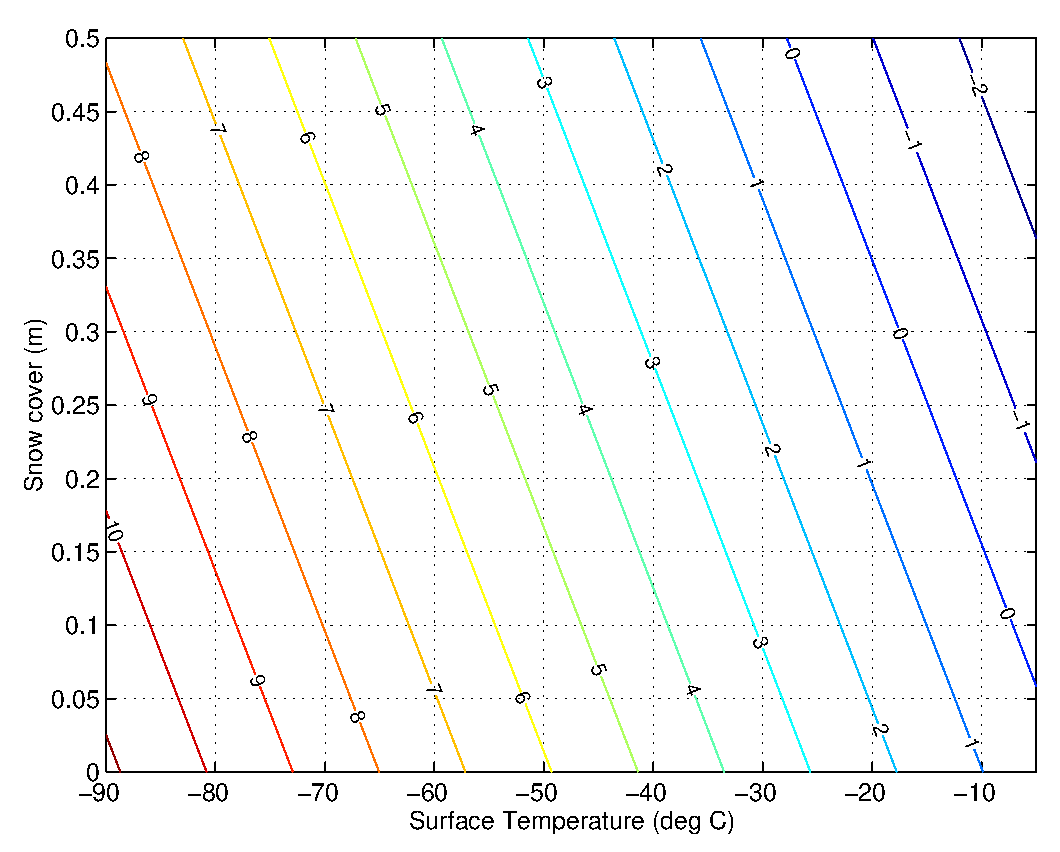
\includegraphics[width=13cm]{heiko/modules_icemod_maxthck}
%\def\epsfsize#1#2{0.8#1}
%\centerline{\vbox{\epsfbox{heiko/modules_icemod_maxthck.ps}}}
\caption[]{Maximal ice floe thickness at a deep sea temperature of $\rm 
2^\circ C$.}
\label{maxthckfig}
\ef

\clearpage
\section*{Ocean heat flux parameterizations}
\label{qoc_obs}
Various parameterizations of the oceanic heat flux $Q_{oc}$ have been
proposed. \cit{Hewitt et al.}{2000}, who use the parameterization proposed by
\cit{Gordon et al.}{2000}, state that they adjust the sea surface temperature 
(SST) such that the oceanic heat flux yields reasonable sea ice concentrations 
and thicknesses. \nocite{hewitt2000} An overview is given in Table 
\ref{flxoctab}. The parameterizations are illustrated in Fig.\ \ref{flxocfig}.
In this work,the coefficient $c_o\, = \rm 0.2\, W\, m^{-2}\, K^{-1}$
 parameterizes the advective oceanic heat transport such that the model
 yields realistic oceanic heat fluxes of $\rm 2\, W\, m^{-2}$ in
 the central arctic and $\rm 10-20\, W\, m^{-2}$ on the latitude of
 Spitzbergen \ct{Hibler and Zhang}{1993}. \nocite{hibler1993}
 
\btbh
\begin{tabular}{lccl}
\hline
Reference & Heat flux ($\rm W\, m^{-2}$) & Parameter values & Model type \\
\hline
this work$^a$                   & $\rm c\, (T_d\, -T_f)$ & $\rm c\,=\,4 (0.4) 
\,W\,m^{-2}\,K^{-1}$     & TD \\
\citp{Cattle and Crossley}{1995}& $\rm \rho_w\, c_{p,w}\, \gamma\, (SST\, 
-T_f)\, /0.5\Delta z_1$ & $\rm \gamma\,=\,2.5\times 10^{-3}\,m^2\,s^{-1}$ & TD 
\\
\citp{Birnbaum}{1998}           & $\rm \rho_w\, c_{p,w}\, \gamma\, u_\ast\, 
(SST\, -T_f)$ & $\rm \gamma\,=\,6\times 10^{-3}$   & D-TD \\
\citp{Lohmann et al.}{1998}     & $\rm c\, (SST\, -T_f)$ & $\rm 
c\,=\,200\,W\,m^{-2}\,K^{-1}$   & TD \\
\citp{Gordon et al.}{2000}      & $\rm c\, (SST\, -T_f)$ & $\rm 
c\,=\,20\,W\,m^{-2}\,K^{-1}$    & TD \\
\citp{Timmermann}{2000}         & $\rm \rho_w\, c_{p,w}\, \gamma\, u_\ast\, 
(SST\, -T_f)$ & $\rm \gamma\,=\,1.2\times 10^{-2}$ & D-TD \\
\citp{Timmermann}{2000}(b)      & $\rm \rho_w\, c_{p,w}\, \gamma\, (SST\, 
-T_f)$ & $\rm \gamma\,=\,10^{-4}\, m\, s^{-1}$ & D-TD \\
\hline
\end{tabular}
\caption[]{Parameterizations of the oceanic heat flux. $\rm T_d,SST$ and $\rm 
T_f$ denote the deep ocean, sea surface and freezing temperature, 
respectively. $\rm \Delta z_1$ denotes the thickness of the uppermost ocean 
box. The considered models are either thermodynamic models (TD) or 
dynamic-thermodynamic models (D-TD). The relative velocity between sea ice 
drift and ocean current is denoted by $u_\ast$. 
$^a$  value for the southern (northern) polar area.}
\label{flxoctab}
\etb
\nocite{cattle1995} \nocite{gordon2000} \nocite{timmermann2000} \nocite{lohmann1998}
\nocite{birnbaum1998}

\begin{figure}[ht]
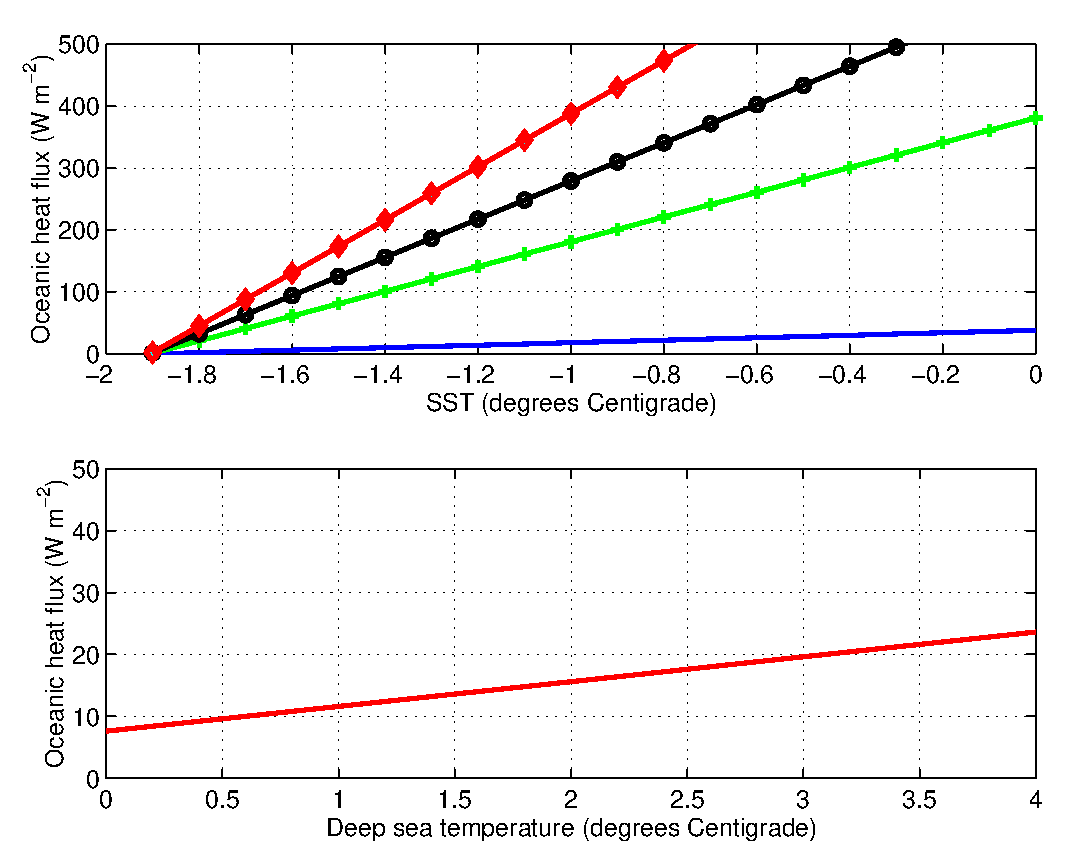
\includegraphics[width=13cm]{heiko/modules_icemod_flxoc}
\caption[]{Parameterizations of the oceanic heat flux. Solid (top): 
\cit{Gordon et al.}{2000}; Solid (bottom): this work (Southern Ocean value). 
Plusses: \cit{Lohmann et al.}{1998}. Circles: \cit{Birnbaum}{1998} with
$\rm u_\ast=8.3\times 10^{-3}$, following \cit{Timmermann}{2000}. Diamonds:
\cit{Cattle and Crossley}{1995} with $\rm \Delta z_1=50\, m$, which then 
yields results equivalent to \citp{Timmermann}{2000}(b).}
\label{flxocfig}
\end{figure}

\clearpage

\section*{Output}
Submodule-specific output is written to tape whenever the namelist
parameter {\em NOUTPUT} is set to 1. An overview of output fields is
given in Table \ref{ice_output}. The scalar values are written in the 
diagnostic routine, i.e. every {\em NDIAG} time steps (default value every
5 days). The global fields are written every {\em NOUT} time steps (default
value every 2 days).


\btbh
\begin{center}
\begin{tabular}{llr}
\hline
Output field & Description & Code \\
\hline
\multicolumn{3}{c}{\em Scalar values written to fort.76 resp. icecover.srv} \\
xarc	& Ice cover Arctic Ocean		& 951 \\
xant	& Ice cover Southern Ocean		& 952 \\
xarcd	& Mean ice thickness Arctic Ocean	& 953 \\
xantd	& Mean ice thickness Southern Ocean	& 954 \\
xarcsnd	& Mean snow depth Arctic Ocean		& 955 \\
xantsnd	& Mean snow depth Southern Ocean	& 956 \\
xarcmf	& Melt/freeze flux Arctic Ocean		& 961 \\
xantmf	& Melt/freeze flux Southern Ocean	& 962 \\
xarcd.clim & Climatological mean ice thickness Arctic Ocean	& 963 \\
xantd.clim & Climatological mean ice thickness Southern Ocean	& 964 \\
\hline
\multicolumn{3}{c}{\em Global fields written to fort.75 resp. icedata.srv} \\
xicec 	& Ice concentration 			& 210 \\
xiced 	& Ice thickness				& 211 \\
xsnow 	& Snow depth				& 141 \\
xcliced2& Climatological ice thickness		& 911 \\
xcmf	& Cumulative melt/freeze flux		& 801 \\
xheat	& Heat flux received from atmosphere	& 701 \\
xqoc	& Heat flux received from deep ocean	& 702 \\
xcflux	& Conductive heat flux passed to ocean	& 703 \\
xfluxrs	& Ice growth flux saved for next time step & 704 \\
fxice2	& Flux correction ice thickness		& 705 \\
xlst	& Land / Sea mask time dependent $^a$	& 972 \\
\hline
\end{tabular}
\end{center}
\label{ice_output}
\caption{Sea ice model output. $^a$ The land sea mask has to be written for
every time step to avoid GRADS problems, as all other variables in 
$icedata.srv$ are time-dependent.}
\etb


\btbh
\begin{center}
\begin{tabular}{llr}
\hline
Output field & Description & Code \\
\hline
ytoc	& SST				& 851 \\
yhmix	& MLD				& 853 \\
yclim2 	& Climatological SST		& 721 \\
ycdpt2 	& Climatological MLD		& 722 \\
yfsst2 	& Flux correction SST		& 711 \\
yfdpt2 	& Flux correction MLD		& 712 \\
ytbottom & Deep ocean temperature	& 852 \\
yqoc 	& Heat flux from deep ocean	& 702 \\
\hline
\end{tabular}
\end{center}
\label{ocean_output}
\caption{Mixed layer model output written to fort.31 resp. oceandata.srv.}
\etb








